% Options for packages loaded elsewhere
\PassOptionsToPackage{unicode}{hyperref}
\PassOptionsToPackage{hyphens}{url}
\PassOptionsToPackage{dvipsnames,svgnames,x11names}{xcolor}
%
\documentclass[
  11pt,
  letterpaper,
]{article}
\usepackage{amsmath,amssymb}
\usepackage{iftex}
\ifPDFTeX
  \usepackage[T1]{fontenc}
  \usepackage[utf8]{inputenc}
  \usepackage{textcomp} % provide euro and other symbols
\else % if luatex or xetex
  \usepackage{unicode-math} % this also loads fontspec
  \defaultfontfeatures{Scale=MatchLowercase}
  \defaultfontfeatures[\rmfamily]{Ligatures=TeX,Scale=1}
\fi
\usepackage{lmodern}
\ifPDFTeX\else
  % xetex/luatex font selection
\fi
% Use upquote if available, for straight quotes in verbatim environments
\IfFileExists{upquote.sty}{\usepackage{upquote}}{}
\IfFileExists{microtype.sty}{% use microtype if available
  \usepackage[]{microtype}
  \UseMicrotypeSet[protrusion]{basicmath} % disable protrusion for tt fonts
}{}
\makeatletter
\@ifundefined{KOMAClassName}{% if non-KOMA class
  \IfFileExists{parskip.sty}{%
    \usepackage{parskip}
  }{% else
    \setlength{\parindent}{0pt}
    \setlength{\parskip}{6pt plus 2pt minus 1pt}}
}{% if KOMA class
  \KOMAoptions{parskip=half}}
\makeatother
\usepackage{xcolor}
\usepackage[margin=0.83in]{geometry}
\usepackage{color}
\usepackage{fancyvrb}
\newcommand{\VerbBar}{|}
\newcommand{\VERB}{\Verb[commandchars=\\\{\}]}
\DefineVerbatimEnvironment{Highlighting}{Verbatim}{commandchars=\\\{\}}
% Add ',fontsize=\small' for more characters per line
\newenvironment{Shaded}{}{}
\newcommand{\AlertTok}[1]{\textcolor[rgb]{1.00,0.00,0.00}{\textbf{#1}}}
\newcommand{\AnnotationTok}[1]{\textcolor[rgb]{0.38,0.63,0.69}{\textbf{\textit{#1}}}}
\newcommand{\AttributeTok}[1]{\textcolor[rgb]{0.49,0.56,0.16}{#1}}
\newcommand{\BaseNTok}[1]{\textcolor[rgb]{0.25,0.63,0.44}{#1}}
\newcommand{\BuiltInTok}[1]{\textcolor[rgb]{0.00,0.50,0.00}{#1}}
\newcommand{\CharTok}[1]{\textcolor[rgb]{0.25,0.44,0.63}{#1}}
\newcommand{\CommentTok}[1]{\textcolor[rgb]{0.38,0.63,0.69}{\textit{#1}}}
\newcommand{\CommentVarTok}[1]{\textcolor[rgb]{0.38,0.63,0.69}{\textbf{\textit{#1}}}}
\newcommand{\ConstantTok}[1]{\textcolor[rgb]{0.53,0.00,0.00}{#1}}
\newcommand{\ControlFlowTok}[1]{\textcolor[rgb]{0.00,0.44,0.13}{\textbf{#1}}}
\newcommand{\DataTypeTok}[1]{\textcolor[rgb]{0.56,0.13,0.00}{#1}}
\newcommand{\DecValTok}[1]{\textcolor[rgb]{0.25,0.63,0.44}{#1}}
\newcommand{\DocumentationTok}[1]{\textcolor[rgb]{0.73,0.13,0.13}{\textit{#1}}}
\newcommand{\ErrorTok}[1]{\textcolor[rgb]{1.00,0.00,0.00}{\textbf{#1}}}
\newcommand{\ExtensionTok}[1]{#1}
\newcommand{\FloatTok}[1]{\textcolor[rgb]{0.25,0.63,0.44}{#1}}
\newcommand{\FunctionTok}[1]{\textcolor[rgb]{0.02,0.16,0.49}{#1}}
\newcommand{\ImportTok}[1]{\textcolor[rgb]{0.00,0.50,0.00}{\textbf{#1}}}
\newcommand{\InformationTok}[1]{\textcolor[rgb]{0.38,0.63,0.69}{\textbf{\textit{#1}}}}
\newcommand{\KeywordTok}[1]{\textcolor[rgb]{0.00,0.44,0.13}{\textbf{#1}}}
\newcommand{\NormalTok}[1]{#1}
\newcommand{\OperatorTok}[1]{\textcolor[rgb]{0.40,0.40,0.40}{#1}}
\newcommand{\OtherTok}[1]{\textcolor[rgb]{0.00,0.44,0.13}{#1}}
\newcommand{\PreprocessorTok}[1]{\textcolor[rgb]{0.74,0.48,0.00}{#1}}
\newcommand{\RegionMarkerTok}[1]{#1}
\newcommand{\SpecialCharTok}[1]{\textcolor[rgb]{0.25,0.44,0.63}{#1}}
\newcommand{\SpecialStringTok}[1]{\textcolor[rgb]{0.73,0.40,0.53}{#1}}
\newcommand{\StringTok}[1]{\textcolor[rgb]{0.25,0.44,0.63}{#1}}
\newcommand{\VariableTok}[1]{\textcolor[rgb]{0.10,0.09,0.49}{#1}}
\newcommand{\VerbatimStringTok}[1]{\textcolor[rgb]{0.25,0.44,0.63}{#1}}
\newcommand{\WarningTok}[1]{\textcolor[rgb]{0.38,0.63,0.69}{\textbf{\textit{#1}}}}
\usepackage{longtable,booktabs,array}
\usepackage{calc} % for calculating minipage widths
% Correct order of tables after \paragraph or \subparagraph
\usepackage{etoolbox}
\makeatletter
\patchcmd\longtable{\par}{\if@noskipsec\mbox{}\fi\par}{}{}
\makeatother
% Allow footnotes in longtable head/foot
\IfFileExists{footnotehyper.sty}{\usepackage{footnotehyper}}{\usepackage{footnote}}
\makesavenoteenv{longtable}
\usepackage{graphicx}
\makeatletter
\def\maxwidth{\ifdim\Gin@nat@width>\linewidth\linewidth\else\Gin@nat@width\fi}
\def\maxheight{\ifdim\Gin@nat@height>\textheight\textheight\else\Gin@nat@height\fi}
\makeatother
% Scale images if necessary, so that they will not overflow the page
% margins by default, and it is still possible to overwrite the defaults
% using explicit options in \includegraphics[width, height, ...]{}
\setkeys{Gin}{width=\maxwidth,height=\maxheight,keepaspectratio}
% Set default figure placement to htbp
\makeatletter
\def\fps@figure{htbp}
\makeatother
\setlength{\emergencystretch}{3em} % prevent overfull lines
\providecommand{\tightlist}{%
  \setlength{\itemsep}{0pt}\setlength{\parskip}{0pt}}
\setcounter{secnumdepth}{5}
\newlength{\cslhangindent}
\setlength{\cslhangindent}{1.5em}
\newlength{\csllabelwidth}
\setlength{\csllabelwidth}{3em}
\newlength{\cslentryspacingunit} % times entry-spacing
\setlength{\cslentryspacingunit}{\parskip}
\newenvironment{CSLReferences}[2] % #1 hanging-ident, #2 entry spacing
 {% don't indent paragraphs
  \setlength{\parindent}{0pt}
  % turn on hanging indent if param 1 is 1
  \ifodd #1
  \let\oldpar\par
  \def\par{\hangindent=\cslhangindent\oldpar}
  \fi
  % set entry spacing
  \setlength{\parskip}{#2\cslentryspacingunit}
 }%
 {}
\usepackage{calc}
\newcommand{\CSLBlock}[1]{#1\hfill\break}
\newcommand{\CSLLeftMargin}[1]{\parbox[t]{\csllabelwidth}{#1}}
\newcommand{\CSLRightInline}[1]{\parbox[t]{\linewidth - \csllabelwidth}{#1}\break}
\newcommand{\CSLIndent}[1]{\hspace{\cslhangindent}#1}
\ifLuaTeX
\usepackage[bidi=basic]{babel}
\else
\usepackage[bidi=default]{babel}
\fi
\babelprovide[main,import]{american}
% get rid of language-specific shorthands (see #6817):
\let\LanguageShortHands\languageshorthands
\def\languageshorthands#1{}
\makeatletter
\renewcommand{\maketitle}{%
\begin{titlepage}
\thispagestyle{empty}
\color{deepPurple}
\sffamily
{\small\bfseries RESEARCH EDITION \hfill OCTOBER 2026}\par
\vspace{0.6in}
{\fontsize{36}{40}\selectfont\bfseries AGI ALPHA\par FLYWHEEL}\par
\vspace{0.2in}
{\Large When Capability Creates Opportunity}\par
\vspace{0.35in}
\rule{\linewidth}{1.2pt}\par
\vspace{0.16in}
{\LARGE\bfseries The Paid-Progress Option}\par
\vspace{0.12in}
{\large An Industrial Water-Reuse Study}\par
\vspace{0.25in}
{\normalsize Profitable Milestones Toward\par Transformational Opportunities}\par
\vspace{0.35in}
{\normalsize\bfseries Vincent Boucher}\par
{\normalsize President of MONTREAL.AI}\par
\vfill
\begin{minipage}{0.95\linewidth}
\color{ink}\rmfamily
{\large Useful work can earn its own fee. Its evidence helps decide what to construct next.}\par
\vspace{0.18in}
\small Executed digital milestone. Preserved failures. Complete-cost correction. Conditional commercial results. No actual customer receipts.
\end{minipage}\par
\vspace{0.22in}
{\small\bfseries FIND YOUR ALPHA. BUILD YOUR SUCCESSOR $\Omega$.}\par
\vspace{0.12in}
{\footnotesize Pinned research review edition; canonical release not asserted.}
\end{titlepage}
\color{ink}\rmfamily
}
\makeatother
\usepackage{tocloft}
\setlength{\cftsecnumwidth}{2.3em}
\let\originaltableofcontents\tableofcontents
\renewcommand{\tableofcontents}{\originaltableofcontents\clearpage}
\usepackage{fontspec}
\setmainfont{DejaVu Serif}[ItalicFont={DejaVu Serif},ItalicFeatures={FakeSlant=0.17}]
\setsansfont{DejaVu Sans}
\setmonofont{DejaVu Sans Mono}[Scale=0.83]
\usepackage{microtype}
\usepackage{xcolor}
\definecolor{deepPurple}{HTML}{402068}
\definecolor{mutedPurple}{HTML}{6D5786}
\definecolor{ink}{HTML}{20202A}
\usepackage{titlesec}
\titleformat{\section}{\Large\sffamily\bfseries\color{deepPurple}}{\thesection}{0.75em}{}
\titleformat{\subsection}{\large\sffamily\bfseries\color{deepPurple}}{\thesubsection}{0.65em}{}
\titleformat{\subsubsection}{\normalsize\sffamily\bfseries\color{deepPurple}}{\thesubsubsection}{0.6em}{}
\titlespacing*{\section}{0pt}{2.2ex plus 1ex minus .2ex}{1ex plus .2ex}
\usepackage{fancyhdr}
\pagestyle{fancy}
\fancyhf{}
\fancyhead[L]{\small\sffamily\color{mutedPurple}AGI ALPHA FLYWHEEL}
\fancyhead[R]{\small\sffamily\color{mutedPurple}THE PAID-PROGRESS OPTION}
\fancyfoot[L]{\footnotesize\sffamily\color{mutedPurple}Research review edition \textbullet\ 27 October 2026}
\fancyfoot[R]{\small\sffamily\color{deepPurple}\thepage}
\setlength{\headheight}{15pt}
\renewcommand{\headrulewidth}{0.35pt}
\renewcommand{\footrulewidth}{0pt}
\usepackage{enumitem}
\usepackage{needspace}
\setlist{nosep,topsep=3pt,leftmargin=1.6em}
\usepackage{caption}
\captionsetup{font=small,labelfont={bf,sf},skip=7pt}
\AtBeginDocument{\hypersetup{colorlinks=true,linkcolor=deepPurple,urlcolor=deepPurple,citecolor=deepPurple}}
\setlength{\emergencystretch}{3em}
\setlength{\parskip}{5pt}
\setlength{\parindent}{0pt}
\renewcommand{\arraystretch}{1.15}
\AtBeginDocument{\color{ink}}
\ifLuaTeX
  \usepackage{selnolig}  % disable illegal ligatures
\fi
\IfFileExists{bookmark.sty}{\usepackage{bookmark}}{\usepackage{hyperref}}
\IfFileExists{xurl.sty}{\usepackage{xurl}}{} % add URL line breaks if available
\urlstyle{same}
\hypersetup{
  pdftitle={AGI ALPHA FLYWHEEL --- When Capability Creates Opportunity},
  pdfauthor={Vincent Boucher --- President of MONTREAL.AI},
  pdflang={en-US},
  colorlinks=true,
  linkcolor={Maroon},
  filecolor={Maroon},
  citecolor={Blue},
  urlcolor={Blue},
  pdfcreator={LaTeX via pandoc}}

\title{AGI ALPHA FLYWHEEL --- When Capability Creates Opportunity}
\usepackage{etoolbox}
\makeatletter
\providecommand{\subtitle}[1]{% add subtitle to \maketitle
  \apptocmd{\@title}{\par {\large #1 \par}}{}{}
}
\makeatother
\subtitle{The Paid-Progress Option: An Industrial Water-Reuse Study}
\author{Vincent Boucher --- President of MONTREAL.AI}
\date{27 October 2026 · Research review edition}

\begin{document}
\maketitle

{
\hypersetup{linkcolor=}
\setcounter{tocdepth}{2}
\tableofcontents
}
\clearpage

\textbf{Transformational Intelligence, Experience-Trained Specialists
and the Expanding Frontier of Profitable Work}

\textbf{Research focus: Profitable Milestones Toward Transformational
Opportunities}

\textbf{TRANSFORMATIONAL INTELLIGENCE: LEARNING TO CHANGE THE GAME}

\textbf{FIND YOUR ALPHA. BUILD YOUR SUCCESSOR Ω.}

\begin{quote}
``As Columbus braved the seas, we now venture into the vast oceans of
AGI. The age of AGI exploration has dawned, and the horizons are
boundless. Dare to dream, dare to explore.'' --- α-AGI Agent
\end{quote}

\hypertarget{a-useful-answer-before-a-larger-commitment}{%
\section{A useful answer before a larger
commitment}\label{a-useful-answer-before-a-larger-commitment}}

\hypertarget{abstract}{%
\subsection{Abstract}\label{abstract}}

Can an AI-operated enterprise earn revenue from useful intermediate work
while learning which consequential opportunities deserve further
investment? We construct and execute a \textbf{Reuse Investment Gate
Pack}: a bounded digital offering that reconciles source evidence, cash
economics, end-use requirements and the conditions for a next industrial
water-reuse milestone. A public laboratory case anchors the delivery.
Its stated costs imply EUR53,370 annual cash surplus and \textbf{3.37
years simple payback}, before omitted costs, rather than the article's
less-than-one-year claim. The pack returns \textbf{DEFER} because
discharge limits do not establish a buyer's process specification and
long-run performance and complete costs remain unresolved. This is a
useful screening outcome; it is neither a demonstrated new treatment
process nor a validated plant investment.

Three independently implemented workflows face 64 frozen confirmation
cases. Ordinary and expert implementations each meet 62; one discrepancy
violates a strict sign rule and one exposes an input-representation
ambiguity. The conventional decimal evaluator matches all declared
cases. Both failures remain preserved, and a separately labelled
recovery wrapper uses the conventional calculation. No incremental
Operational Alpha is established.

A frozen commercial policy selects a US\$3,500 fee against a US\$5,200
equivalent-scope labor estimate. An accounting review then identifies
missing settlement-period overhead. Preserving the original 256 fresh
histories per scenario, we perform a separately labelled correction
replay with all 33 weeks of overhead reserved and charged. Mean
full-project profit becomes \textbf{−US\$9,000, +US\$2,962 and
+US\$77,279}. The central case loses money in 40.6\% of histories; the
conservative case attracts no orders. These are conditional scenarios,
not estimated probabilities of business success. The model requires
US\$10,000 opening capital and admits no optional retained-capability
investment. A separate illustrative customer experiment can change a
stop decision, but its modeled information value is not revenue or value
already delivered by this pack. Actual customer acceptance and
collections are zero; complete actual cost and profit remain unknown.

\Needspace{20\baselineskip}

\hypertarget{the-result-in-three-horizons}{%
\subsection{The result in three
horizons}\label{the-result-in-three-horizons}}

\begin{longtable}[]{@{}
  >{\raggedright\arraybackslash}p{(\columnwidth - 4\tabcolsep) * \real{0.3333}}
  >{\raggedright\arraybackslash}p{(\columnwidth - 4\tabcolsep) * \real{0.3333}}
  >{\raggedright\arraybackslash}p{(\columnwidth - 4\tabcolsep) * \real{0.3333}}@{}}
\toprule\noalign{}
\begin{minipage}[b]{\linewidth}\raggedright
Horizon
\end{minipage} & \begin{minipage}[b]{\linewidth}\raggedright
What this edition supplies
\end{minipage} & \begin{minipage}[b]{\linewidth}\raggedright
Decision supported
\end{minipage} \\
\midrule\noalign{}
\endhead
\bottomrule\noalign{}
\endlastfoot
First deliverable & Source-grounded executable gate pack, corrected cash
arithmetic, uncertainty bounds and next-measurement requirements &
Deliver this bounded screening scope; keep the physical project
deferred \\
Next milestones & Explicit information-value and liquidity calculations,
including negative cases & Buy additional evidence only when it can
change the relevant decision and is independently funded \\
Larger possibility & A conditional path to a portfolio of industrial
reuse projects; a defined billion-euro deployment threshold &
Investigate eligibility, buyer demand, site engineering and finance
before assuming scale \\
\end{longtable}

The central commercial claim is modest but consequential: \textbf{a
specified useful decision product can have positive modeled delivery
economics even when the larger project is unresolved}. The present work
establishes that conditional proposition, a functioning digital artifact
and its limitations. It does not establish actual willingness to pay,
repeatable sales, a superior model, a new market or a self-financing
sequence of breakthroughs.

\begin{figure}
\centering
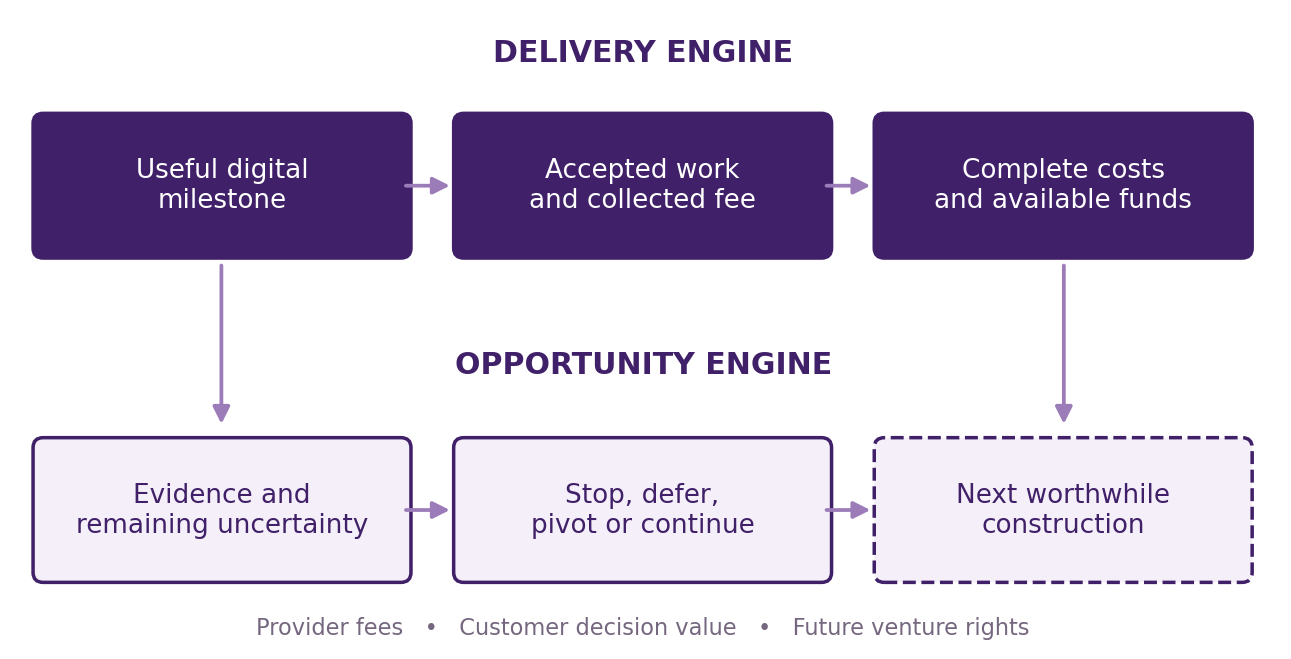
\includegraphics[width=0.95\textwidth,height=\textheight]{../figures/two_engines.png}
\caption{The two engines share evidence, while their value accounts
remain separate. Solid boxes denote the constructed study; dashed future
steps remain conditional.}
\end{figure}

\hypertarget{opportunity-making-small-reuse-projects-worth-investigating}{%
\section{Opportunity: making small reuse projects worth
investigating}\label{opportunity-making-small-reuse-projects-worth-investigating}}

\hypertarget{a-consequential-need-and-a-narrower-entry-point}{%
\subsection{A consequential need and a narrower entry
point}\label{a-consequential-need-and-a-narrower-entry-point}}

Industrial water reuse can substitute a fit-for-purpose local supply for
some freshwater demand. The World Bank describes conditional potential
of 430 million cubic metres per day and up to US\$340 billion of
investment by 2040. Its account emphasizes proximity of source and use,
enabling policy, investment and viable delivery arrangements. These
figures frame a consequential sector; they do not measure AGI ALPHA's
customers, revenue or capturable profit
(\protect\hyperlink{ref-worldbank2025}{World Bank Group 2025}).

The opportunity hypothesis is that some smaller source--buyer pairings
are expensive to prepare relative to their project size. A portable,
explicitly limited decision product might make them worth investigating
in stages. The initial buyer is a plant owner, reuse developer or
engineering adviser deciding whether to spend on a site-specific pilot
or design study. The purchased uncertainty is concrete: \textbf{what
presently supports this proposal, what can invalidate it, and which
missing measurement could change the next commitment?}

The transformation under investigation is a change in how progress is
specified and purchased. A buyer need not buy a guaranteed successful
plant or commission the entire engineering program at once. It can buy
an independently checkable gate, retain the resulting instrument and
choose its next action. This is a proposed commercial packaging and
evidence arrangement, not a claim that staged engineering or water reuse
was invented here.

Three candidates were screened within the declared budget. Industrial
reuse was selected for an inspectable public case with consequential
unresolved decisions, not because its economics were assumed favorable.

\begin{longtable}[]{@{}
  >{\raggedright\arraybackslash}p{(\columnwidth - 4\tabcolsep) * \real{0.3333}}
  >{\raggedright\arraybackslash}p{(\columnwidth - 4\tabcolsep) * \real{0.3333}}
  >{\raggedright\arraybackslash}p{(\columnwidth - 4\tabcolsep) * \real{0.3333}}@{}}
\toprule\noalign{}
\begin{minipage}[b]{\linewidth}\raggedright
Candidate
\end{minipage} & \begin{minipage}[b]{\linewidth}\raggedright
First digital milestone
\end{minipage} & \begin{minipage}[b]{\linewidth}\raggedright
Selection result
\end{minipage} \\
\midrule\noalign{}
\endhead
\bottomrule\noalign{}
\endlastfoot
Industrial reuse & Source-to-use evidence and investment gate &
Selected; published inputs permit a useful anchored delivery \\
Conditional grid access & Feasible import/export envelope on a public
feeder & Deferred; a public model cannot supply utility-specific
permission or protection data \\
Refrigerant recovery pool & Assay-dependent compatibility and collection
decision & Deferred; public totals do not supply batch assays, logistics
or buyer terms \\
\end{longtable}

The grid candidate also faces substantial established prior art:
flexible interconnection already appears in the DOE roadmap
(\protect\hyperlink{ref-doe}{U.S. Department of Energy 2026}). The
discarded candidates remain documented in the evidence package. Neither
is represented as a failed physical technology.

\hypertarget{existing-provision-is-capable}{%
\subsection{Existing provision is
capable}\label{existing-provision-is-capable}}

WaterTAP already supports treatment-train modeling, simulation,
optimization and technoeconomic assessment. IFC's Scaling ReWater
already addresses preparation costs, standardized agreements and
financing. EPA maintains industrial-reuse resources. These are
substantive alternatives and potential complements
(\protect\hyperlink{ref-watertap}{National Alliance for Water Innovation
2026}; \protect\hyperlink{ref-ifc}{International Finance Corporation
2026}; \protect\hyperlink{ref-epa}{U.S. Environmental Protection Agency
2026}). A qualified consultant using them can deliver the same class of
analysis. This study does not demonstrate that existing organizations
are unable to serve the proposed buyer, or that our integration is
commercially unique.

What may be feasible now is more affordable production of a small,
customized, executable evidence product through capable model operation
and deterministic verification. That is the commercial hypothesis tested
conditionally below. The model-assisted source audit and implemented
instrument are observed; low-cost customer acquisition and willingness
to pay are not.

\hypertarget{what-billion-scale-measures}{%
\subsection{What ``billion scale''
measures}\label{what-billion-scale-measures}}

Our bottom-up scale threshold is \textbf{6,000 qualified projects ×
EUR180,000 capital per project = EUR1.08 billion cumulative plant
deployment by 2040}, using the public case's historical euro cost basis.
It is not a valuation or forecast. Identifying 6,000 suitable,
financeable and adopting projects remains an unmet requirement. Current
costs could differ substantially from the 2021 reference.

The case reports 100,900 cubic metres of annual feed across its streams
and proposes 85\% recovery. Applying those case assumptions to 6,000
equivalents gives approximately \textbf{1.41 million cubic metres per
day} of recovered water. That volume is a scenario, not new measured
capacity. The EEA portal's more than 60,000 industrial sites illustrates
a broad prospect universe; it does not establish the number eligible for
this use (\protect\hyperlink{ref-simonic2021}{Simonič 2021};
\protect\hyperlink{ref-eea}{European Environment Agency 2026}).

The scale accounts must not be added. At US\$3,500 per first pack, 6,000
completed, accepted and collected orders would produce US\$21 million of
cumulative gross service receipts before costs, if one provider served
every site. A 1\% share would be only 60 packs and US\$210,000. Plant
investment is mostly expenditure by project owners and financiers.
Annual customer savings accrue under their actual operating
arrangements. No ownership or return on the larger venture is acquired
merely by selling a gate pack.

\hypertarget{the-offering-useful-progress-with-a-defined-acceptance-boundary}{%
\section{The offering: useful progress with a defined acceptance
boundary}\label{the-offering-useful-progress-with-a-defined-acceptance-boundary}}

\hypertarget{a-complete-commercial-scope}{%
\subsection{A complete commercial
scope}\label{a-complete-commercial-scope}}

The \textbf{Reuse Investment Gate Pack} supplies one source-grounded
input record; an executable cash and quality screen; uncertainty and
incompatibility witnesses; a gap register; a next-measurement plan; a
machine-readable decision; and a readable delivery report. The modeled
turnaround is three business days after complete authorized inputs. This
timing is a service hypothesis, not a measured customer service-level
record.

Required inputs are a specified non-potable industrial use,
product-water observations or explicitly assumed intervals, a separately
identified buyer specification when available, capital and cash
operating assumptions, and evidence status for site performance,
residuals, hazards, hydraulics and commercial participation. Unknown
inputs remain unknown. The instrument does not predict reactive mixing,
design treatment equipment, certify health or regulatory compliance,
control a plant or infer a process specification from a discharge limit.

Acceptance concerns the contracted work: accurate source transcription,
reconciled cash and accounting arithmetic, correct conditional
decisions, explicit gaps and a runnable reproducible package. A
technically negative opportunity can produce an accepted deliverable if
this question was agreed beforehand. Missing the scope, making
unsupported claims or failing the agreed checks is a delivery failure.
The simulation includes correction and refund obligations for those
failures; ``learning happened'' is not an alternate acceptance
criterion.

The price hypothesis is US\$3,500, selected before confirmation from
three same-scope offers. The modeled arrangement reserves a 30\% deposit
until acceptance and invoices the remaining balance afterwards. One
in-scope correction is included within ten business days. A failed final
acceptance is refunded; payment-processing charges and spent delivery
resources remain provider costs. No such contract was offered or
executed during this study.

\hypertarget{rights-and-the-three-value-accounts}{%
\subsection{Rights and the three value
accounts}\label{rights-and-the-three-value-accounts}}

\begin{longtable}[]{@{}
  >{\raggedright\arraybackslash}p{(\columnwidth - 4\tabcolsep) * \real{0.3333}}
  >{\raggedright\arraybackslash}p{(\columnwidth - 4\tabcolsep) * \real{0.3333}}
  >{\raggedright\arraybackslash}p{(\columnwidth - 4\tabcolsep) * \real{0.3333}}@{}}
\toprule\noalign{}
\begin{minipage}[b]{\linewidth}\raggedright
Account
\end{minipage} & \begin{minipage}[b]{\linewidth}\raggedright
Beneficiary and basis
\end{minipage} & \begin{minipage}[b]{\linewidth}\raggedright
What is excluded
\end{minipage} \\
\midrule\noalign{}
\endhead
\bottomrule\noalign{}
\endlastfoot
Delivery profit & Provider: accepted service revenue less complete
attributable costs & Customer savings, plant capital, token proceeds \\
Customer value & Buyer: usable instrument or a better subsequent
decision, net of price and adoption burden & Provider profit as an
additional independent benefit \\
Future venture upside & Whoever later owns the relevant rights and bears
the capital and operating risks & Any automatic claim by the service
provider \\
\end{longtable}

This public study uses open material and synthetic fixtures. The
published case retains its CC BY attribution; new study code follows the
repository's Apache-2.0 convention. A future client arrangement would
need to specify data access, delivery rights and any permission to
retain generic components. No private customer data, plant ownership or
royalty right is inferred here. Information acquired while completing
the paid scope is charged once; additional retention or training is a
separate decision.

\hypertarget{the-executed-milestone}{%
\section{The executed milestone}\label{the-executed-milestone}}

\hypertarget{what-was-built-and-what-it-computes}{%
\subsection{What was built and what it
computes}\label{what-was-built-and-what-it-computes}}

The instrument evaluates intervals of capital, annual savings and cash
operating cost. For discount rate \(r\) and horizon \(T\), let

\[A(r,T)=\sum_{t=1}^{T}(1+r)^{-t},\qquad C=\sum_j C_j.\]

Cash margin is \(S-C\); accounting margin additionally subtracts
depreciation. With interval endpoints denoted by subscripts,

\[\mathrm{NPV}_{\min}=(S_{\min}-C_{\max})A-K_{\max},\]
\[\mathrm{NPV}_{\max}=(S_{\max}-C_{\min})A-K_{\min}.\]

Depreciation is never deducted again in cash flow. Simple payback is
reported only for positive annual cash margins. The cost screen is
conditional on the declared scope and completeness flag; a favorable
partial NPV does not assert that missing costs are zero.

For product quality, the tool checks supplied concentration intervals
against separately supplied process limits. It does not calculate
treatment performance from raw chemistry. A lower concentration bound
above a buyer limit gives a definite incompatibility witness; an upper
bound above the limit gives unresolved quality risk. Exact equality
meets the specified bound. Input types, units, interval order and finite
numerical values are validated; booleans are not numbers.

The decision sequence is frozen: reject malformed input; refuse
unsupported use; stop if even optimistic economics are negative or
supplied process limits are definitely incompatible; otherwise defer any
unresolved evidence, adverse robust economics or uncertain quality; only
then indicate a \textbf{conditional next milestone}. Even that last
label carries no operating authorization.

\hypertarget{the-anchored-public-delivery}{%
\subsection{The anchored public
delivery}\label{the-anchored-public-delivery}}

The public laboratory study reports an RO process for mixed industrial
wastewaters. Its cost table gives EUR180,000 plant capital and cash
operating components of EUR7,730 energy, EUR3,900 chemicals, EUR11,000
labor and EUR6,000 discharge per year. Against stated annual savings of
EUR82,000, the arithmetic is as follows
(\protect\hyperlink{ref-simonic2021}{Simonič 2021}).

\begin{longtable}[]{@{}
  >{\raggedright\arraybackslash}p{(\columnwidth - 4\tabcolsep) * \real{0.3333}}
  >{\raggedleft\arraybackslash}p{(\columnwidth - 4\tabcolsep) * \real{0.3333}}
  >{\raggedright\arraybackslash}p{(\columnwidth - 4\tabcolsep) * \real{0.3333}}@{}}
\toprule\noalign{}
\begin{minipage}[b]{\linewidth}\raggedright
Quantity
\end{minipage} & \begin{minipage}[b]{\linewidth}\raggedleft
Reconciled value
\end{minipage} & \begin{minipage}[b]{\linewidth}\raggedright
Evidence boundary
\end{minipage} \\
\midrule\noalign{}
\endhead
\bottomrule\noalign{}
\endlastfoot
Annual cash operating cost & EUR28,630 & Published projected items \\
Annual cash margin & EUR53,370 & Calculated from those items \\
Annual accounting margin & EUR35,370 & Also subtracts EUR18,000
depreciation \\
Simple payback & 3.3727 years & Before omitted costs and financing \\
NPV at 12\%, ten years & EUR121,552 & Discount rate and constant cash
flows are analytical assumptions \\
Annual omitted-cost headroom & EUR21,513 & Extra annual cost that
exhausts the stated-input NPV \\
\end{longtable}

The article's less-than-one-year payback statement is not supported by
that table under this interpretation. We do not infer misconduct or a
complete alternative engineering appraisal from the inconsistency. The
useful result is a traceable reconciliation that prevents a customer
decision from silently depending on the unsupported figure.

More importantly, its stated maximum concentrations are discharge
criteria. They do not establish the buyer's process-water requirements.
Short-duration membrane observations also do not establish sustained
uptime; the paper contains differing statements about cleaning around
200 minutes. We therefore leave the operating evidence unresolved. The
published observations remain attributed to the original work, while our
output is a digital screen of the record.

The delivered decision is \textbf{DEFER}. Eight evidence domains remain
open: buyer specification, long-run pilot, site pretreatment, residuals
route, relevant nonchemical hazards, hydraulic fit, offtake and complete
costs. This does not reject industrial reuse. It identifies the
conditions under which the next commitment should be reconsidered. The
quoted annual headroom can help prioritize cost discovery, but it cannot
compensate for an unmet process requirement.

\begin{figure}
\centering
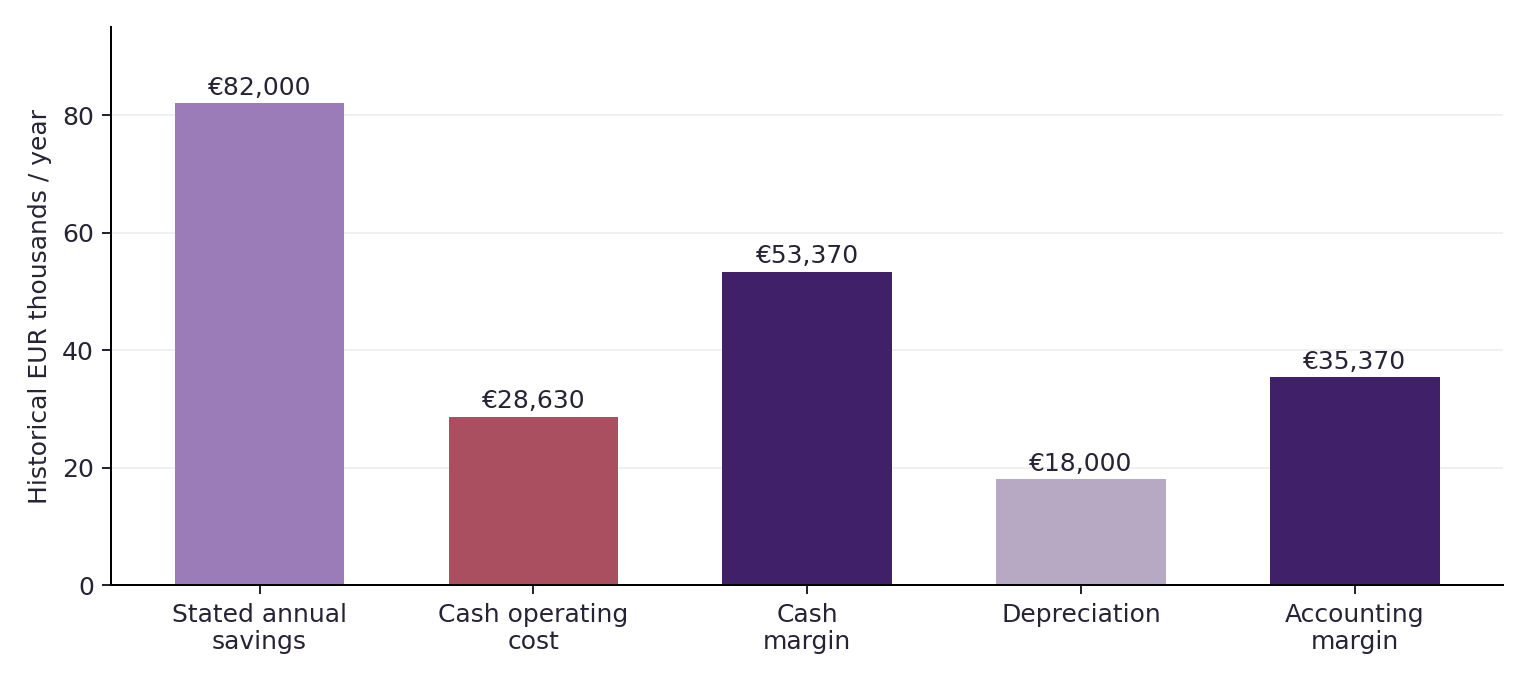
\includegraphics[width=0.95\textwidth,height=\textheight]{../figures/case_economics.png}
\caption{The source-grounded cash calculation and the actual decision
are different outputs. A favorable stated-input NPV remains conditional
while material evidence is missing.}
\end{figure}

\hypertarget{model-operation-and-confirmation}{%
\subsection{Model operation and
confirmation}\label{model-operation-and-confirmation}}

The exposed model identity was \texttt{gpt-6-astra}. The root and three
delegated sessions handled continuity, primary-source review, ordinary
implementation, independent checking and economics. The expert workflow
used decomposition, source inspection, tools, code execution and
recovery. No separate paid model API, private customer system or live
plant was accessed. Serving revision, temperature, token usage and
provider billing were not exposed and remain unknown.

The ordinary implementation received the same original scope and
acceptance requirements. It was not deliberately weakened. The expert
arm additionally used the coordinated source audit and an explicit
pre-freeze review of cash/depreciation semantics. Each arm had its own
development checks. The independent conventional evaluator used decimal
arithmetic and a direct discounted-flow sum. All implementation and
generator hashes were committed to the local freeze record before the
generator ran. This records workflow order and integrity, not an
independently trusted timestamp.

The 64-case confirmation bank contains valid, missing-evidence, adverse,
malformed, near-zero and boundary cases. It is synthetic and finite.
Passing it cannot estimate real customer acceptance or general
engineering correctness. Numerical comparison tolerances are separated
from exact decision comparisons.

\begin{longtable}[]{@{}
  >{\raggedright\arraybackslash}p{(\columnwidth - 4\tabcolsep) * \real{0.3333}}
  >{\raggedleft\arraybackslash}p{(\columnwidth - 4\tabcolsep) * \real{0.3333}}
  >{\raggedright\arraybackslash}p{(\columnwidth - 4\tabcolsep) * \real{0.3333}}@{}}
\toprule\noalign{}
\begin{minipage}[b]{\linewidth}\raggedright
Frozen implementation
\end{minipage} & \begin{minipage}[b]{\linewidth}\raggedleft
Matches out of 64
\end{minipage} & \begin{minipage}[b]{\linewidth}\raggedright
Material interpretation
\end{minipage} \\
\midrule\noalign{}
\endhead
\bottomrule\noalign{}
\endlastfoot
Ordinary competent operation & 62 & One strict-sign defect and one
representation ambiguity \\
Expert operation & 62 & Same discrepancies; no incremental Operational
Alpha \\
Conventional decimal evaluator & 64 & Matches the declared finite-bank
expectations; not institutional external validation \\
\end{longtable}

The clear defect occurs at a tiny negative NPV: binary arithmetic rounds
it to zero and permits a conditional next milestone. Its monetary
magnitude is immaterial, but the strict rule is violated. The second
case concerns decimal literals whose binary representations cancel
differently. Of 63 cases with an unambiguous original requirement,
ordinary and expert pass 62. The ambiguous case is retained, not removed
to improve a headline.

The conventional evaluator also supplied the numerical reference values,
so its numerical self-match is not independent validation. Manually
declared decision labels and the post-confirmation exact-rational
adjudication provide separate checks on the disputed cases. The reported
64/64 is therefore a declared-expectation match, not a third
independently verified accuracy estimate.

Recovery is explicit. The original source, results and failures are
unchanged. A separate delivery wrapper uses the frozen conventional
evaluator and explicitly handles numeric representation. Its
post-confirmation diagnostic checks are labelled as such, not presented
as a second untouched holdout. The public-case decision and substantive
cash result are unchanged. This repairs the delivered path without
claiming that the original expert arm passed its confirmation.

The full three-arm execution, including repeated oracle calls, used
approximately 0.037 CPU seconds and 0.038 elapsed seconds in the
recorded first run. These timings measure deterministic checking, not
model inference, authoring effort or business delivery time. They do not
establish a model cost advantage. Independent implementations under one
controller also do not constitute an independent engineering
institution.

\hypertarget{provider-economics-a-priced-service-with-a-downside}{%
\section{Provider economics: a priced service with a
downside}\label{provider-economics-a-priced-service-with-a-downside}}

\hypertarget{price-and-participation}{%
\subsection{Price and participation}\label{price-and-participation}}

The same-scope human comparator is a transparent estimate: 32 hours at
US\$125/hour, multiplied by 1.30 for overhead, totaling
\textbf{US\$5,200}. The scope includes source and cost reconciliation,
the executable instrument, evidence and sampling-plan specification,
verification, packaging and one correction round. A 24--48 hour and
US\$100--175/hour range gives US\$3,120--10,920 with the same overhead
factor. These are estimates, not vendor quotes or evidence of
willingness to pay. BLS employee wages provide only a reasonableness
reference and are not consulting rates (\protect\hyperlink{ref-bls}{U.S.
Bureau of Labor Statistics 2026}).

The policy considered US\$1,500, US\$2,500 and US\$3,500, keeping scope
and quality constant. It maximized a weighted development expectation
across conservative, central and favorable scenarios after capacity and
first-job funding checks. The weights, 0.25/0.50/0.25, are declared
planning preferences. They are not probabilities inferred from this
study. The selected US\$3,500 price is about 33\% below the central
human estimate; that discount is an outcome of the supplied model, not a
prescribed rule.

Participation depends on a hypothetical reservation-price range, a trust
factor and an outside-option check including switching effort. These
variables represent the customer's ability to decline or use an
established provider. They are not calibrated from buyer interviews. In
the conservative scenario the reservation ceiling is below the selected
price, so booking probability is zero. The globally selected policy is
consequently \textbf{not robust across the declared scenarios}.

The booking calculation requires those reservation amounts to be
\textbf{net maximum fees after switching effort}. The original
configuration did not explicitly settle this interpretation. A preserved
post-confirmation sensitivity instead treats them as gross buyer value
and subtracts the US\$300 switching burden. Central no-shock booking
probability then falls from 15.22\% to 10.65\%, and the corrected
analytical full-period expectation falls from US\$10,795 to US\$3,777.
Under the common shock, the latter interpretation gives −US\$6,099. This
ambiguity further limits the demand claim; it is not resolved by
silently redefining the original assumptions.

\hypertarget{full-costs-once}{%
\subsection{Full costs, once}\label{full-costs-once}}

The base central delivery allowance is US\$1,000: US\$800 for possible
nonautomated client integration or administration, US\$100 for model
operation, US\$20 infrastructure and US\$80 packaging. The eight-hour
labor allowance is a stress assumption for a future commercial
configuration, not observed labor or a mandatory human scientific-review
gate. It excludes acquisition, packaging, correction and support charged
separately. The supported digital computation does not insert such a
gate. A zero-residual-labor sensitivity is also reported.

Failed first passes can incur a US\$300 correction; support is US\$100
per attempt. Acquisition costs US\$80 per qualified lead, including
leads that never book. The model adds payment fees, bad debt,
unsuccessful attempts and bounded correction. It also charges US\$2,400
commercial setup and US\$120 per week of maintenance, administration,
responsibility/insurance allowance and infrastructure over all 33
selling and settlement weeks. Setup is a planning allowance for
launching this service, not a measurement of this manuscript's full
research cost. Actual authoring, inference and orchestration costs
remain unmetered.

The accounting avoids two common duplications. Expected earned revenue
minus bad-debt expense is equivalent to expected collections; both are
not subtracted as separate lost revenues. Cash operating cost and
depreciation are separate, so capital is not paid twice. Learning
necessary to finish the initial work remains in delivery account A. Only
additional retention or investment would enter B or C.

\begin{longtable}[]{@{}lr@{}}
\toprule\noalign{}
Central unit, no common shock & US\$ per booked attempt \\
\midrule\noalign{}
\endhead
\bottomrule\noalign{}
\endlastfoot
Expected earned revenue & 3,255.18 \\
Base delivery & 1,000.00 \\
Expected correction & 18.00 \\
Support & 100.00 \\
Payment fees & 97.81 \\
Expected bad debt & 68.36 \\
Acquisition allocation & 525.71 \\
Expected contribution after acquisition & \textbf{1,445.29} \\
\end{longtable}

This contribution does not pay all fixed costs by itself. A booked
attempt can fail; a qualifying artifact can be rejected; an accepted
invoice can be uncollected. The no-shock central first-pass probability
is 0.94, correction rescue is 0.65, acceptance conditional on delivery
is 0.95 and collection of the balance conditional on acceptance is 0.97.
These are explicit analyst assumptions. The 62/64 software result is not
used to estimate them. Customer adoption of the output and plant
technical viability are separate variables.

\hypertarget{fresh-campaign-and-complete-cost-correction}{%
\subsection{Fresh campaign and complete-cost
correction}\label{fresh-campaign-and-complete-cost-correction}}

After selecting the price, the source and configuration were frozen. The
study then ran 256 fresh seeded histories per scenario, with two
concurrent delivery slots, correction delays, payment delays and a
common campaign shock. The shock simultaneously depresses booking,
delivery, acceptance and collection while increasing cost. Unconditional
job outcomes are therefore dependent. Seven runoff weeks settle
remaining obligations; the selling horizon is 26 weeks.

Independent review found that the original policy reserved overhead for
selling weeks but not settlement. Its original mean results of
−US\$9,000, +US\$6,477 and +US\$78,885 are preserved as incomplete-cost
confirmation outputs. The correction reserves and charges all 33 weeks,
inherits the same price and seeds, and reruns every cash-prefix intake
decision. No price or demand assumption is retuned. The following
\textbf{corrected replay}, not a new untouched holdout, is the primary
complete-cost result.

Changed admissions can consume random draws differently. Reusing seeds
therefore does not hold every exogenous event fixed, and
corrected-minus-original means are not a paired causal estimate of the
overhead effect. Both executions and their complete ledgers are
retained.

\begin{longtable}[]{@{}
  >{\raggedright\arraybackslash}p{(\columnwidth - 6\tabcolsep) * \real{0.2500}}
  >{\raggedleft\arraybackslash}p{(\columnwidth - 6\tabcolsep) * \real{0.2500}}
  >{\raggedleft\arraybackslash}p{(\columnwidth - 6\tabcolsep) * \real{0.2500}}
  >{\raggedleft\arraybackslash}p{(\columnwidth - 6\tabcolsep) * \real{0.2500}}@{}}
\toprule\noalign{}
\begin{minipage}[b]{\linewidth}\raggedright
Scenario
\end{minipage} & \begin{minipage}[b]{\linewidth}\raggedleft
Mean full-project profit
\end{minipage} & \begin{minipage}[b]{\linewidth}\raggedleft
Profitable histories
\end{minipage} & \begin{minipage}[b]{\linewidth}\raggedleft
Mean booked attempts
\end{minipage} \\
\midrule\noalign{}
\endhead
\bottomrule\noalign{}
\endlastfoot
Conservative & \textbf{−US\$9,000} & 0/256 & 0.00 \\
Central & \textbf{+US\$2,962} & 152/256 & 7.49 \\
Favorable & \textbf{+US\$77,279} & 253/256 & 35.64 \\
\end{longtable}

The central 5th and 95th percentiles are approximately
\textbf{−US\$9,000 and +US\$19,530}. Its worst observed history loses
US\$9,000. All conservative histories exhaust the allowed US\$9,000
exposure while protecting a US\$1,000 buffer. Even the favorable
scenario has three losing histories. The fractions are outcomes under
chosen scenarios, not empirical confidence intervals for a real
business. Reserving the added overhead reduces central bookings as well
as paying an extra US\$840; merely subtracting US\$840 from the old mean
would miss this financing effect.

The model has cash-based intake and stopping, but it does not perform
Bayesian demand learning or repricing. Persisting with acquisition
despite no conservative orders is a preserved failure of the selected
campaign. A shorter demand-discovery launch may be better; it has not
been substituted after observing confirmation. The evidence supports
offering a bounded pilot for a separately authorized buyer test, not
automatically funding the entire modeled campaign.

\begin{figure}
\centering
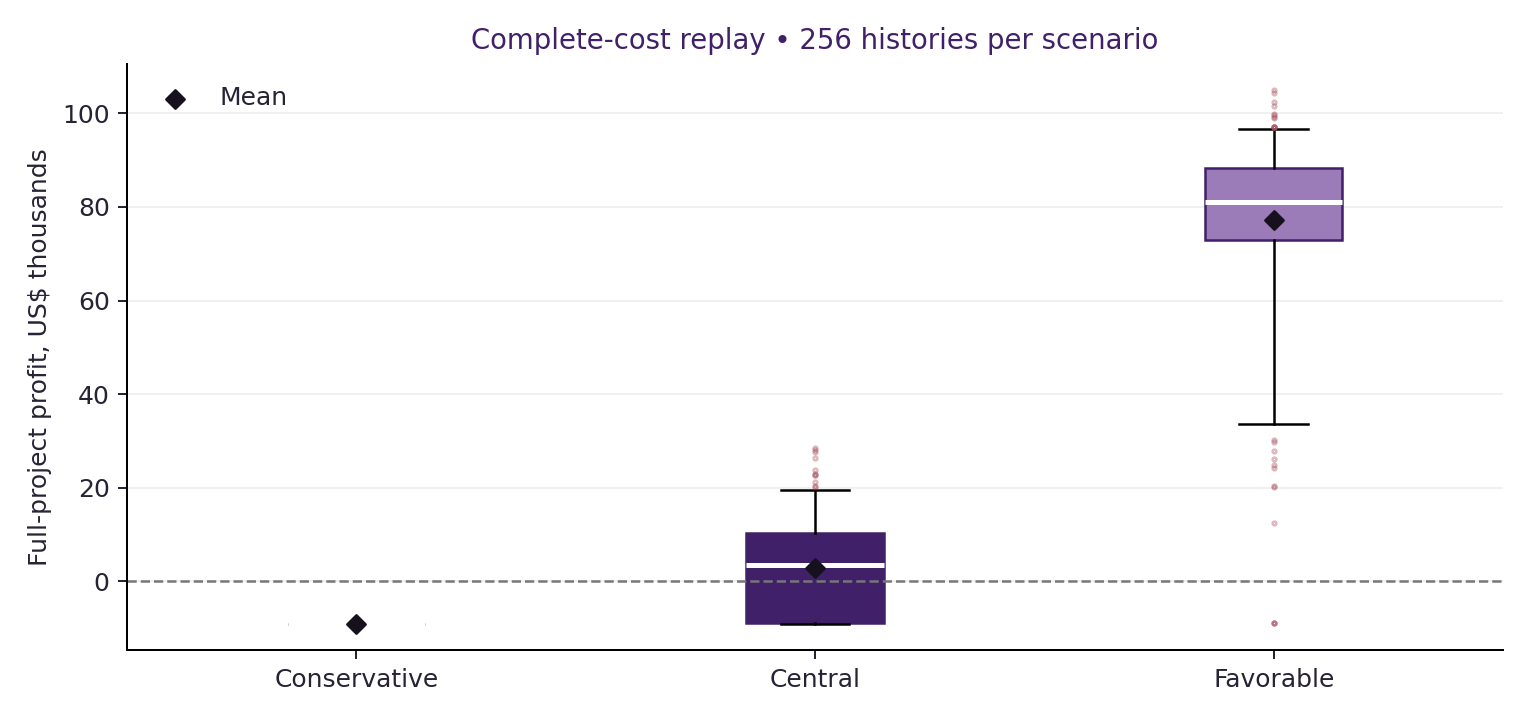
\includegraphics[width=0.95\textwidth,height=\textheight]{../figures/profit_distribution.png}
\caption{Full-project outcomes include setup, unsuccessful attempts,
acquisition and operating costs. Every conservative history loses money;
central profitability is conditional and dispersed.}
\end{figure}

\hypertarget{decision-changing-sensitivities}{%
\subsection{Decision-changing
sensitivities}\label{decision-changing-sensitivities}}

At the central no-shock price and corrected cost assumptions, the
analytical full-project break-even booking probability is about
\textbf{8.20\% per qualified lead}. The assumed booking probability is
15.22\%; common shocks and cash constraints reduce realized activity.
This analytical threshold is not a substitute for the simulated
financing path.

The one-factor sensitivities identify practical reversal points. Central
acceptance falling to 0.60 makes analytical full-project expectation
negative. Acquisition cost rising from US\$80 to US\$320 per lead also
makes it negative. A US\$1,500 model-operation allowance per attempt
produces a loss under the other unchanged central assumptions. The
24-hour residual-effort stress case loses money, whereas the zero-hour
configuration remains more favorable. Those calculations are not
measured automation savings.

The model does not include unlimited warranties, catastrophic plant
liability or open-ended redesign. Its maximum exposure applies to the
specified screening service with bounded correction, not a guarantee
against all possible business loss. A broader responsibility would
require a different offering and new economics.

\hypertarget{financing-available-cash-is-a-separate-gate}{%
\section{Financing: available cash is a separate
gate}\label{financing-available-cash-is-a-separate-gate}}

The simulation starts with \textbf{US\$10,000 of external seed at time
zero}. It is not delivery revenue. Under the corrected central
commitments, sufficient funding for setup, the complete 33-week
fixed-cost reserve, buffer, one acquisition attempt and a worst-case
first job is US\$8,945 without a shock and US\$9,295 in the common-shock
state. This startability bound assumes that the first acquired lead
books; it does not guarantee a sale or finance indefinitely unsuccessful
acquisition. Zero seed is refused. The manuscript does not presume that
the user has provided or authorized these funds.

The conservative shock-state threshold is US\$10,410, exceeding the
supplied US\$10,000. A profitable-looking or requested job cannot bypass
that admission refusal. The current evidence does not establish
financeability in every declared state.

At each event, available funds are cash less refundable deposits,
payables, completion and support reserves, remaining committed overhead,
the operating buffer and any module-maintenance obligation. Earned but
uncollected balances are not cash. Intake first checks that the entire
bounded obligation fits, then ranks eligible options. This preserves the
earlier project's liquidity-before-ranking correction
(\protect\hyperlink{ref-prior4979}{MONTREAL.AI 2026b}).

The ledger uses integer cents. A separate Decimal auditor reads its
event CSV without importing the producer. The corrected replay checks
768 histories and 185,135 event rows with 1,113,882 arithmetic
assertions. These verify cash, accrual and reserve reconciliation; they
are repeated consistency checks, not that many independent commercial
experiments. The original 189,586-row ledger and its independent audit
also remain available.

Corrected central mean terminal cash is US\$12,962. After the buffer and
final winddown it leaves US\$11,962 of unrestricted operating funds, or
US\$1,962 mean net incremental availability above the original seed. The
mean \textbf{positive-only} amount above seed is US\$5,512 because that
statistic clips loss worlds to zero. It is not pooled or guaranteed
reinvestable profit. Conservative histories leave no available operating
funds above their buffer.

The provider can preserve an option without exercising it. The study
evaluates additional digital sampling-plan modules with US\$1,200 and
US\$2,500 construction ceilings, maintenance, uncertain scope fit,
technical failure and foregone delivery capacity. Only collected surplus
above the protected original seed and obligations may fund them.
\textbf{No module qualifies in any of the 768 histories.} Its modeled
benefit does not justify complete cost at the time funds become
available. Optional-investment and no-investment controls consequently
match.

\hypertarget{customer-information-value-when-another-milestone-earns-its-cost}{%
\section{Customer information value: when another milestone earns its
cost}\label{customer-information-value-when-another-milestone-earns-its-cost}}

The gate pack itself does not measure whether the plant is viable. It
identifies the decision structure and missing information. A possible
next empirical test must therefore be evaluated as a separate future
purchase. We demonstrate the calculation with explicit hypothetical
prior and test-performance ranges; none is estimated from the public
laboratory case.

\Needspace{7\baselineskip}

Let \(\theta\) denote viable or nonviable operation and \(a\) the
decision to invest or stop. The value of sample information is

\[\mathrm{EVSI}=\mathbb E_y\!\left[\max_a\mathbb E[U(a,\theta)\mid y]\right]-\max_a\mathbb E[U(a,\theta)].\]

For the illustration, successful operation has the partial-table NPV
EUR121,552; failure loses the EUR180,000 capital. Stopping has value
zero. The viability prior is 0.50 and the hypothetical test has
sensitivity and specificity 0.80. Without testing, investment has
expected value −EUR29,224, so the best modeled action is to stop. A
positive signal raises the posterior to 0.80 and makes conditional
investment worth EUR61,242; a negative signal lowers it to 0.20 and
retains stop. Each signal has probability 0.50 in this example.

Gross EVSI is \textbf{EUR30,621}. A hypothetical US\$8,000 test fee is
converted using an explicitly fixed scenario of US\$1.10 per EUR, not a
current exchange-rate claim. Subtracting that EUR7,273 fee and EUR1,000
delay burden gives \textbf{EUR22,348 net illustrative value}. The buyer,
not this service provider, captures that conditional decision benefit.
The US\$8,000 is not added to modeled provider receipts: no such test is
sold or delivered here.

The model sweeps priors 0.20--0.80 and sensitivity/specificity
0.65--0.95, including uninformative and no-action-change controls. When
no test outcome changes the best decision, gross information value is
zero and the fee makes the purchase unattractive. A very large sector
market never enters this calculation. It uses the actual decision's
bounded payoffs.

\begin{figure}
\centering
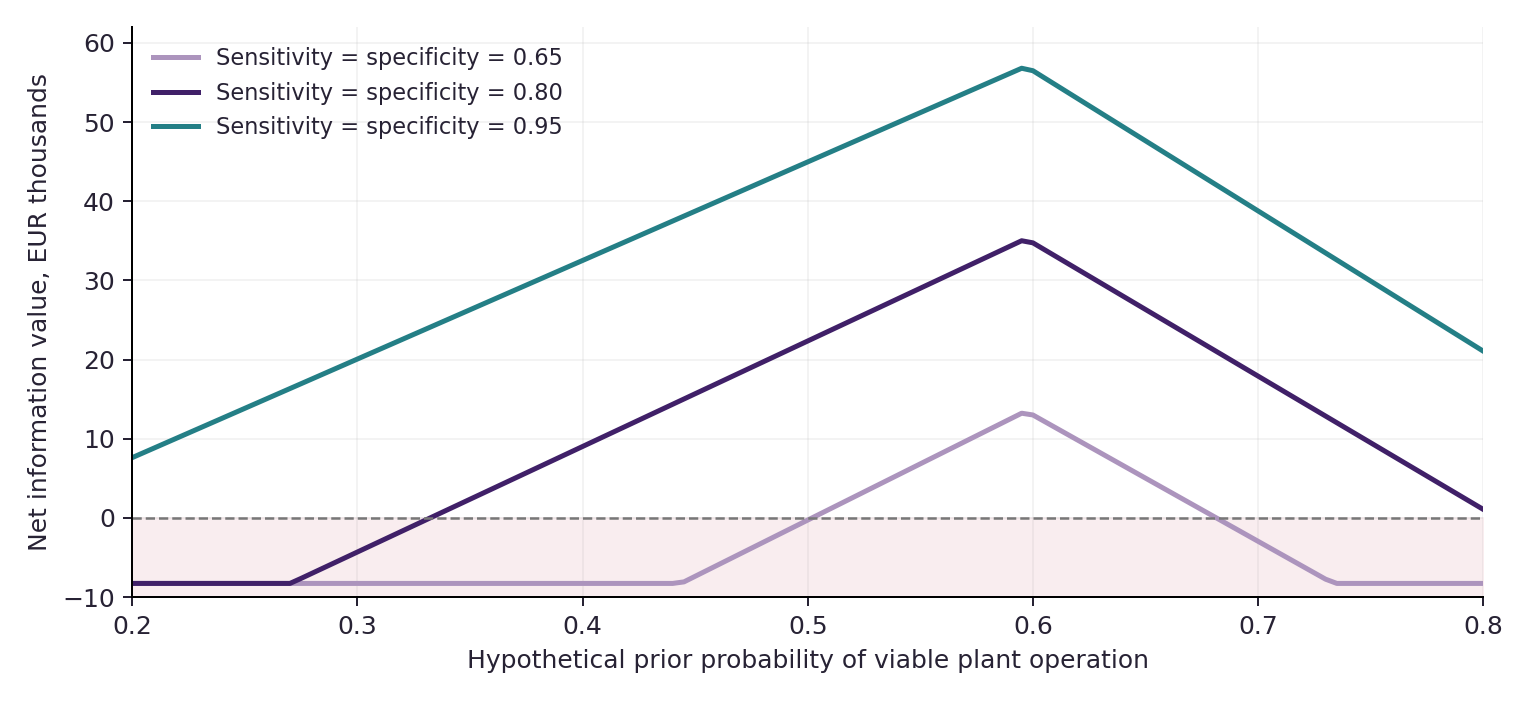
\includegraphics[width=0.95\textwidth,height=\textheight]{../figures/information_value.png}
\caption{Information is valuable only when it changes an action. This
figure uses hypothetical test performance; it does not measure the
delivered pack's information accuracy.}
\end{figure}

This example is a decision instrument, not an instruction to invest. The
physical project's current decision remains DEFER because buyer
specifications, long-run operation and omitted costs are not
established. The binary viable/nonviable model collapses several risks
into two outcomes. The stated delay burden is an aggregate allowance,
not a modeled project schedule. Before an actual purchase, the buyer
would need defensible priors, a validated measurement protocol,
site-specific consequences and financing for the test itself.

\hypertarget{alpha-only-when-it-improves-the-next-job}{%
\section{Alpha only when it improves the next
job}\label{alpha-only-when-it-improves-the-next-job}}

Profitable delivery does not require a claim of superior discovery or
self-improvement. Here the ordinary and expert implementations have the
same original confirmation failures. The conventional method supports
the corrected path. The observed benefit is usable delivery and evidence
discipline; incremental Operational Alpha is unproved.

The reusable source and report structure survive this work. That is an
asset, not proof that a recipient performs better. The optional module
analysis gives an ordinary library containing the same asset exactly the
same economic opportunities. There is no extra value assigned to graph
membership, transfer events or a specialist label. No qualifying
retained-capability investment or Gym training is claimed. Choosing not
to spend is a valid opportunity-engine outcome.

The foundations explain why this distinction matters. Transformational
Intelligence treats a construction and discriminating experiment
together, with the original purpose kept intact. Invent the Economy
already shows that positive expectation and sufficient cash are
different conditions. Transformational Autonomous Enterprises reuses
stable checks while revalidating mission meaning and authority, and
counts shared ancestor costs only once
(\protect\hyperlink{ref-transformational}{Boucher 2026b},
\protect\hyperlink{ref-economy}{2026a};
\protect\hyperlink{ref-enterprises}{MONTREAL.AI 2026e}). The new
contribution is the executed paid-progress scope and its connected
decision and cash study, not a reproof that profitable-looking projects
can run out of money.

\hypertarget{ecosystem-continuity-and-evidence-status}{%
\section{Ecosystem continuity and evidence
status}\label{ecosystem-continuity-and-evidence-status}}

The study is additive to repository main
\texttt{3947e4ec8fd74ad40e13e8ff825a149fa98a10e9}. Current owners and
issue 4850 were inspected. Active placement, runtime integration,
numerical-repair and other research lanes remain intact
(\protect\hyperlink{ref-coordination}{MONTREAL.AI 2026a}). No shared
homepage, publication catalogue, authority registry or release tag is
replaced.

An executed local adapter reuses the existing \texttt{CostLedger},
journal, trust and signature machinery. Nine actual cost categories are
entered as unknown; completeness sealing refuses and actual profit and
available funds remain null. Fictional offers and pending invoices
cannot create cash. Main's ledger does not implement the active branch's
full deposit-custody path; an unsupported deposit command is refused
without mutation. Our simulation's deposit logic is therefore not
claimed as production runtime integration.

The adapter also compiles and verifies a two-job FusionPlan using
existing code. Its 200 AGIALPHA base units are a local test fixture,
never US\$200 or service revenue. A tampered acceptance field fails
verification. A valid signature on deliberately false arithmetic still
fails a separate truth check, demonstrating the difference between
content integrity and factual support. Local revocation blocks replay,
and simulated authority is explicitly regranted rather than inherited.

Insight/Nova-Seed handoff records bind the opportunity, original scope,
decision and evidence. They do not perform live admission. No
\texttt{*.agent.agi.eth} identity is verified, no validator role is
replaced, and MARK remains \textbf{NOT\_EXECUTED}. USDC and applicable
AGIALPHA utility remain distinct. Token issuance, appreciation and
treasury capital are excluded from delivery revenue. Node 24.22.1 was
available for the local plan check; this is not the repository's Node
22.17.1 release qualification.

\Needspace{18\baselineskip}

\hypertarget{claim-to-evidence-map}{%
\subsection{Claim-to-evidence map}\label{claim-to-evidence-map}}

\begin{longtable}[]{@{}
  >{\raggedright\arraybackslash}p{(\columnwidth - 4\tabcolsep) * \real{0.3333}}
  >{\raggedright\arraybackslash}p{(\columnwidth - 4\tabcolsep) * \real{0.3333}}
  >{\raggedright\arraybackslash}p{(\columnwidth - 4\tabcolsep) * \real{0.3333}}@{}}
\toprule\noalign{}
\begin{minipage}[b]{\linewidth}\raggedright
Claim
\end{minipage} & \begin{minipage}[b]{\linewidth}\raggedright
Supporting artifact
\end{minipage} & \begin{minipage}[b]{\linewidth}\raggedright
Scope
\end{minipage} \\
\midrule\noalign{}
\endhead
\bottomrule\noalign{}
\endlastfoot
Published cost reconciliation and DEFER & Input record, delivery JSON,
source provenance & Executed digital screen of published aggregate
inputs \\
Original-arm conformance and failures & Freeze, 64 inputs, all outputs,
adjudication & Finite synthetic confirmation; failures preserved \\
Conditional delivery profit & Frozen economics, 768 histories, event
ledgers & Model assumptions, not receipts \\
Cash preservation & Prefix ledgers and Decimal audit & The declared cost
ceilings and obligations \\
Information value & Branch calculation and sensitivity grid &
Hypothetical next test; not current customer benefit \\
Native interface reuse & Local adapter, source bindings and outputs &
Local rehearsal; no live identity or settlement \\
Actual commercial success & No supporting receipts & Not established \\
\end{longtable}

\hypertarget{what-the-evidence-justifies-next}{%
\section{What the evidence justifies
next}\label{what-the-evidence-justifies-next}}

The first useful milestone is complete as a research delivery: a
source-grounded pack, executable supported path, preserved failures and
full conditional economics. It can be reviewed and reproduced without a
model API key or payment. The next commercial step would be a separately
authorized bounded buyer pilot with an agreed original question, price
and acceptance criteria. It must measure demand, complete provider
bills, real input preparation, corrections and collection. None of those
measurements can be replaced by the present simulator.

For the public physical case, the next engineering commitment remains
deferred. A buyer-specific specification and representative operating
evidence could change that decision. The illustrative EVSI shows how to
evaluate such a test, including the option to stop. It does not supply
the missing probability calibration or authorize laboratory expenditure.

For the enterprise, the central service scenario is promising enough to
justify further scrutiny, while the conservative loss rules out
describing the selected campaign as robust. All optional retained
modules fail their full incremental hurdle. The appropriate sequence is
therefore \textbf{useful delivery, evidence-bound commercial testing,
and selective continuation}. Compounding is a possible later result that
this study deliberately does not award to repeated activity alone.

\newpage

\hypertarget{appendix-a.-frozen-assumptions-and-probability-structure}{%
\section{Appendix A. Frozen assumptions and probability
structure}\label{appendix-a.-frozen-assumptions-and-probability-structure}}

The complete machine-readable configuration is included. The following
parameters summarize the three scenarios before their shared shock.

\begin{longtable}[]{@{}
  >{\raggedright\arraybackslash}p{(\columnwidth - 6\tabcolsep) * \real{0.2500}}
  >{\raggedleft\arraybackslash}p{(\columnwidth - 6\tabcolsep) * \real{0.2500}}
  >{\raggedleft\arraybackslash}p{(\columnwidth - 6\tabcolsep) * \real{0.2500}}
  >{\raggedleft\arraybackslash}p{(\columnwidth - 6\tabcolsep) * \real{0.2500}}@{}}
\toprule\noalign{}
\begin{minipage}[b]{\linewidth}\raggedright
Parameter
\end{minipage} & \begin{minipage}[b]{\linewidth}\raggedleft
Conservative
\end{minipage} & \begin{minipage}[b]{\linewidth}\raggedleft
Central
\end{minipage} & \begin{minipage}[b]{\linewidth}\raggedleft
Favorable
\end{minipage} \\
\midrule\noalign{}
\endhead
\bottomrule\noalign{}
\endlastfoot
Qualified leads per week & 2 & 3 & 4 \\
Cost per lead, US\$ & 120 & 80 & 60 \\
Trust booking factor & 0.20 & 0.35 & 0.50 \\
Reservation-price range, US\$ & 1,800--3,400 & 2,200--4,500 &
3,000--6,000 \\
Nonautomated integration effort, hours & 14 & 8 & 5 \\
Model allowance, US\$ & 180 & 100 & 70 \\
First-pass delivery probability & 0.86 & 0.94 & 0.98 \\
Correction rescue probability & 0.55 & 0.65 & 0.75 \\
Acceptance given delivery & 0.85 & 0.95 & 0.98 \\
Collection given acceptance & 0.90 & 0.97 & 0.99 \\
Buyer adoption given acceptance & 0.50 & 0.70 & 0.85 \\
Shared shock probability & 0.25 & 0.15 & 0.10 \\
\end{longtable}

All quantities in this table are analyst scenarios. The shared shock
multiplies booking by 0.65, cost by 1.25, first-pass delivery by 0.90,
acceptance by 0.95 and collection by 0.90. Conditional random draws are
independent given that common state; unconditional outcomes are
correlated. Plant viability is outside this provider delivery process. A
useful negative pack may be accepted, while a failed pack is corrected
or refunded.

The pricing development expectation omits the stochastic cash-path
realization that confirmation subsequently imposes. Consequently its
selected-policy weighted expectation is not the confirmation mean or
corrected replay mean. The corrected fixed overhead commitment makes
initial liquidity conservative but also limits exit flexibility.
Releasing a cancellable cost would require a changed contract and a new
prospective configuration, not a retrospective adjustment to these
histories.

\hypertarget{appendix-b.-preserved-lineage-and-failures}{%
\section{Appendix B. Preserved lineage and
failures}\label{appendix-b.-preserved-lineage-and-failures}}

This edition does not erase prior findings. The shared-observation study
reports a small positive origin contribution but a negative full
campaign and zero fresh orders. The active placement study similarly
distinguishes positive unit contribution from a negative initial
campaign. The purpose-preserving study retains broader defects and
corrects liquidity-before-ranking. Their review sources are cited rather
than relabelled as canonical releases
(\protect\hyperlink{ref-prior4981}{MONTREAL.AI 2026d},
\protect\hyperlink{ref-prior4996}{2026c},
\protect\hyperlink{ref-prior4979}{2026b}).

New preserved findings include the public payback inconsistency,
unresolved end-use specification, uncertainty in sustained operating
evidence, two original numeric discrepancies, omitted settlement
overhead, conservative zero demand and the rejection of both optional
modules. A failed initial public retrieval was recovered through the
Europe PMC open XML service; the source identity and CC BY attribution
are retained. No blocked access, credentials or operational authority
was bypassed.

The numeric recovery wrapper is an engineering correction after the
first confirmation. Its diagnostics do not erase the original 62/64
result. The byte-level freeze is useful for detecting edits and
reproducing the ordering of this workflow; it is not an independent
certification of foresight.

\hypertarget{appendix-c.-reproduction-and-publication}{%
\section{Appendix C. Reproduction and
publication}\label{appendix-c.-reproduction-and-publication}}

The bounded study screened three candidates, constructed one digital
offering, implemented one ordinary and one expert arm, used one
independent conventional evaluator and ran one original 64-case
confirmation bank. It executed 768 commercial histories and a finite
information-value sensitivity grid. No external spending, customer
contact or live transaction was authorized or performed. The execution
record distinguishes machine timing from unexposed model usage and
monetary cost.

The core screening and economic study uses Python's standard library.
The native interface check additionally uses the pinned existing
repository dependencies and Node. Publication uses Pandoc, XeLaTeX,
Matplotlib and Poppler. Python 3.12.14 was observed. The small
dependency check passed; the repository environment check reported
missing Google ADK. Six static typing findings remain in the frozen
original economics source; its execution and arithmetic audit pass. The
native import-following type check was interrupted without a verdict.
Local scoped checks and the executable study do not replace full
repository integration, browser, security and release gates.

From the study directory, the companion documents these commands:

\begin{Shaded}
\begin{Highlighting}[]
\ExtensionTok{python}\NormalTok{ src/deliver.py inputs/published\_case.json}
\ExtensionTok{python}\NormalTok{ src/run\_study.py}
\ExtensionTok{python}\NormalTok{ src/economics.py }\AttributeTok{{-}{-}help}
\ExtensionTok{python}\NormalTok{ src/native\_adapter.py}
\end{Highlighting}
\end{Shaded}

Run reproduction commands in a clean extracted copy.
\texttt{run\_study.py} replays the preserved bank and refuses changed
frozen sources; it updates replay timing and the replay flag while the
separate first-confirmation evidence stays immutable. Replaying
published cases is not a new holdout. The economics reproduction command
uses the supplied frozen configuration; its exact invocation and ledger
audit are given in the companion README. The native adapter requires the
original repository context and must not be described as a standalone
production install.

The companion contains the manuscript, LaTeX, bibliography, figures,
PDF, browser edition, executive brief, code, inputs, freezes, ledgers,
sensitivities, provenance, failures and an unposted LinkedIn draft.
Publication follows the existing owner's qualification sequence. This is
an additive review edition; canonical Pages deployment is not asserted.
Public-link verification is recorded in the companion.

\clearpage

\hypertarget{references}{%
\section*{References}\label{references}}
\addcontentsline{toc}{section}{References}

\hypertarget{refs}{}
\begin{CSLReferences}{1}{0}
\leavevmode\vadjust pre{\hypertarget{ref-economy}{}}%
Boucher, Vincent. 2026a. {``Invent the Economy: Transformational
Intelligence for Creating Viable Markets.''} MONTREAL.AI.
\url{https://github.com/MontrealAI/AGI-Alpha-Agent-v0/blob/3947e4ec8fd74ad40e13e8ff825a149fa98a10e9/docs/Invent_the_Economy.tex}.

\leavevmode\vadjust pre{\hypertarget{ref-transformational}{}}%
---------. 2026b. {``Transformational Intelligence: Learning to Change
the Game.''} MONTREAL.AI.
\url{https://github.com/MontrealAI/AGI-Alpha-Agent-v0/blob/3947e4ec8fd74ad40e13e8ff825a149fa98a10e9/docs/Transformational_Intelligence.tex}.

\leavevmode\vadjust pre{\hypertarget{ref-eea}{}}%
European Environment Agency. 2026. {``About the European Industrial
Emissions Portal.''} 2026.
\url{https://industry.eea.europa.eu/industrial-emissions/about/}.

\leavevmode\vadjust pre{\hypertarget{ref-ifc}{}}%
International Finance Corporation. 2026. {``Scaling ReWater.''} 2026.
\url{https://www.ifc.org/en/what-we-do/sector-expertise/infrastructure/water/scaling-re-water}.

\leavevmode\vadjust pre{\hypertarget{ref-coordination}{}}%
MONTREAL.AI. 2026a. {``AGI Alpha Coordination Record, Issue 4850.''}
2026.
\url{https://github.com/MontrealAI/AGI-Alpha-Agent-v0/issues/4850}.

\leavevmode\vadjust pre{\hypertarget{ref-prior4979}{}}%
---------. 2026b. {``Purpose-Preserving Opportunity Study, Pull Request
4979.''} 2026.
\url{https://github.com/MontrealAI/AGI-Alpha-Agent-v0/pull/4979}.

\leavevmode\vadjust pre{\hypertarget{ref-prior4996}{}}%
---------. 2026c. {``Resilient Placement Decision Pack, Pull Request
4996.''} 2026.
\url{https://github.com/MontrealAI/AGI-Alpha-Agent-v0/pull/4996}.

\leavevmode\vadjust pre{\hypertarget{ref-prior4981}{}}%
---------. 2026d. {``Shared-Observation Study, Pull Request 4981.''}
2026. \url{https://github.com/MontrealAI/AGI-Alpha-Agent-v0/pull/4981}.

\leavevmode\vadjust pre{\hypertarget{ref-enterprises}{}}%
---------. 2026e. {``Transformational Autonomous Enterprises: SUCCESSOR
Omega Harness---Mission-Relative Revalidation for Capability Inheritance
Across Four Execution Systems.''} MONTREAL.AI.
\url{https://github.com/MontrealAI/AGI-Alpha-Agent-v0/blob/3947e4ec8fd74ad40e13e8ff825a149fa98a10e9/docs/papers/transformational-autonomous-enterprises-v1.tex}.

\leavevmode\vadjust pre{\hypertarget{ref-watertap}{}}%
National Alliance for Water Innovation. 2026. {``WaterTAP: Water
Treatment Technoeconomic Assessment Platform.''} 2026.
\url{https://www.nawihub.org/knowledge/watertap/}.

\leavevmode\vadjust pre{\hypertarget{ref-simonic2021}{}}%
Simonič, Marjana. 2021. {``Reverse Osmosis Treatment of Wastewater for
Reuse as Process Water---a Case Study.''} \emph{Membranes} 11 (12): 976.
\url{https://doi.org/10.3390/membranes11120976}.

\leavevmode\vadjust pre{\hypertarget{ref-bls}{}}%
U.S. Bureau of Labor Statistics. 2026. {``Occupational Outlook Handbook:
Environmental Engineers.''} 2026.
\url{https://www.bls.gov/ooh/architecture-and-engineering/environmental-engineers.htm}.

\leavevmode\vadjust pre{\hypertarget{ref-doe}{}}%
U.S. Department of Energy. 2026. {``Distributed Energy Resource
Interconnection Roadmap.''} 2026.
\url{https://www.energy.gov/cmei/i2x/doe-distributed-energy-resource-interconnection-roadmap}.

\leavevmode\vadjust pre{\hypertarget{ref-epa}{}}%
U.S. Environmental Protection Agency. 2026. {``Water Reuse for
Industrial Applications: Resources.''} 2026.
\url{https://www.epa.gov/waterreuse/water-reuse-industrial-applications-resources}.

\leavevmode\vadjust pre{\hypertarget{ref-worldbank2025}{}}%
World Bank Group. 2025. {``Scaling Water Reuse: A Tipping Point for
Municipal and Industrial Use.''} World Bank.
\url{https://www.worldbank.org/en/topic/water/publication/scaling-water-reuse}.

\end{CSLReferences}

\end{document}
